%% LyX 2.0.5.1 created this file.  For more info, see http://www.lyx.org/.
%% Do not edit unless you really know what you are doing.
\documentclass[english]{beamer}
\usepackage{mathptmx}
\usepackage[T1]{fontenc}
\usepackage[latin9]{inputenc}
\usepackage{amsmath}
\usepackage{amssymb}
\usepackage{graphicx}

\makeatletter

%%%%%%%%%%%%%%%%%%%%%%%%%%%%%% LyX specific LaTeX commands.
%% A simple dot to overcome graphicx limitations
\newcommand{\lyxdot}{.}


%%%%%%%%%%%%%%%%%%%%%%%%%%%%%% Textclass specific LaTeX commands.
 % this default might be overridden by plain title style
 \newcommand\makebeamertitle{\frame{\maketitle}}%
 \AtBeginDocument{
   \let\origtableofcontents=\tableofcontents
   \def\tableofcontents{\@ifnextchar[{\origtableofcontents}{\gobbletableofcontents}}
   \def\gobbletableofcontents#1{\origtableofcontents}
 }
 \long\def\lyxframe#1{\@lyxframe#1\@lyxframestop}%
 \def\@lyxframe{\@ifnextchar<{\@@lyxframe}{\@@lyxframe<*>}}%
 \def\@@lyxframe<#1>{\@ifnextchar[{\@@@lyxframe<#1>}{\@@@lyxframe<#1>[]}}
 \def\@@@lyxframe<#1>[{\@ifnextchar<{\@@@@@lyxframe<#1>[}{\@@@@lyxframe<#1>[<*>][}}
 \def\@@@@@lyxframe<#1>[#2]{\@ifnextchar[{\@@@@lyxframe<#1>[#2]}{\@@@@lyxframe<#1>[#2][]}}
 \long\def\@@@@lyxframe<#1>[#2][#3]#4\@lyxframestop#5\lyxframeend{%
   \frame<#1>[#2][#3]{\frametitle{#4}#5}}
 \def\lyxframeend{} % In case there is a superfluous frame end

%%%%%%%%%%%%%%%%%%%%%%%%%%%%%% User specified LaTeX commands.
\usetheme{Warsaw}
%\usetheme{Boadilla}
% or ...

\usecolortheme{orchid}
\setbeamertemplate{footline}[text line]{} % makes the footer EMPTY

\setbeamercovered{transparent}
% or whatever (possibly just delete it)


\usepackage{bbm}

\makeatother

\usepackage{babel}
\begin{document}

\title{Statistical Analysis of a Bike Sharing Transportation System}


\author{J.~Raimbault$^{1,2}$}


\institute{$^{1}$Erasmus Mundus Master in Complex Systems Science, Ecole Polytechnique\\
$^{2}$LVMT, Ecole Nationale des Ponts et Chauss�es}


\date{Therapeutic Evaluation and Complex Systems\\
Oral Presentation\\
December 18, 2013}

\makebeamertitle

\lyxframeend{}\lyxframe{Outline}

\tableofcontents{}


\lyxframeend{}\section{Introduction}


\lyxframeend{}\lyxframe{Bike-sharing systems}

\vfill{}

\begin{itemize}
\item New flexible and ecological transportation system (\cite{demaio2009bike})
? Complementarity to other urban transportation modes (\cite{midgley2009role})
\end{itemize}
\vfill{}

\begin{itemize}
\item Understanding the mechanisms is necessary for its good management
(ex optimizing redistribution process) but also has intrinsic value
(urban life patterns)
\end{itemize}
\vfill{}

\begin{itemize}
\item Many top-down approaches: statistical models (\cite{borgnat2009studying,borgnat2009modelisation},\cite{michau2011peut})
or data-mining analysis (\cite{o2013mining},\cite{vogel2011understanding,kaltenbrunner2010urban})
\end{itemize}
\vfill{}



\lyxframeend{}\lyxframe{Objectives of the project}

\vfill{}

\begin{itemize}
\item Study of Paris' system (Vlib) \cite{nair2013large}
\end{itemize}
\vfill{}

\begin{itemize}
\item Statistical analysis of a large set of real data, general and with
specific purposes (e. g. parametrisation of an ABM), using existing
or new methods
\end{itemize}
\vfill{}

\begin{itemize}
\item At the beginning, apply TE evaluation to relocation system but many
issues.
\end{itemize}
\vfill{}



\lyxframeend{}\section{Data collection}


\lyxframeend{}\lyxframe{Type and origin of data}

\vfill{}

\begin{itemize}
\item Public data provided by the operator in real time. Problem: need a
constantly running collection data process, and only docking station
status (limited information).
\end{itemize}
\vfill{}

\begin{itemize}
\item Why not ask full travel data to operator ? Independant and open research
(\cite{banos2013HDR} ), reporting bias (in \cite{nair2013large}
results are not presented complete because company did not want for
commercial reasons). We do a compromise, and see if we can however
have good results.
\end{itemize}
\vfill{}

\begin{itemize}
\item Also risk of inconscious spin in the description of results \cite{boutron2010reporting}
\end{itemize}
\vfill{}



\lyxframeend{}\lyxframe{Data collection process}

\hfill{}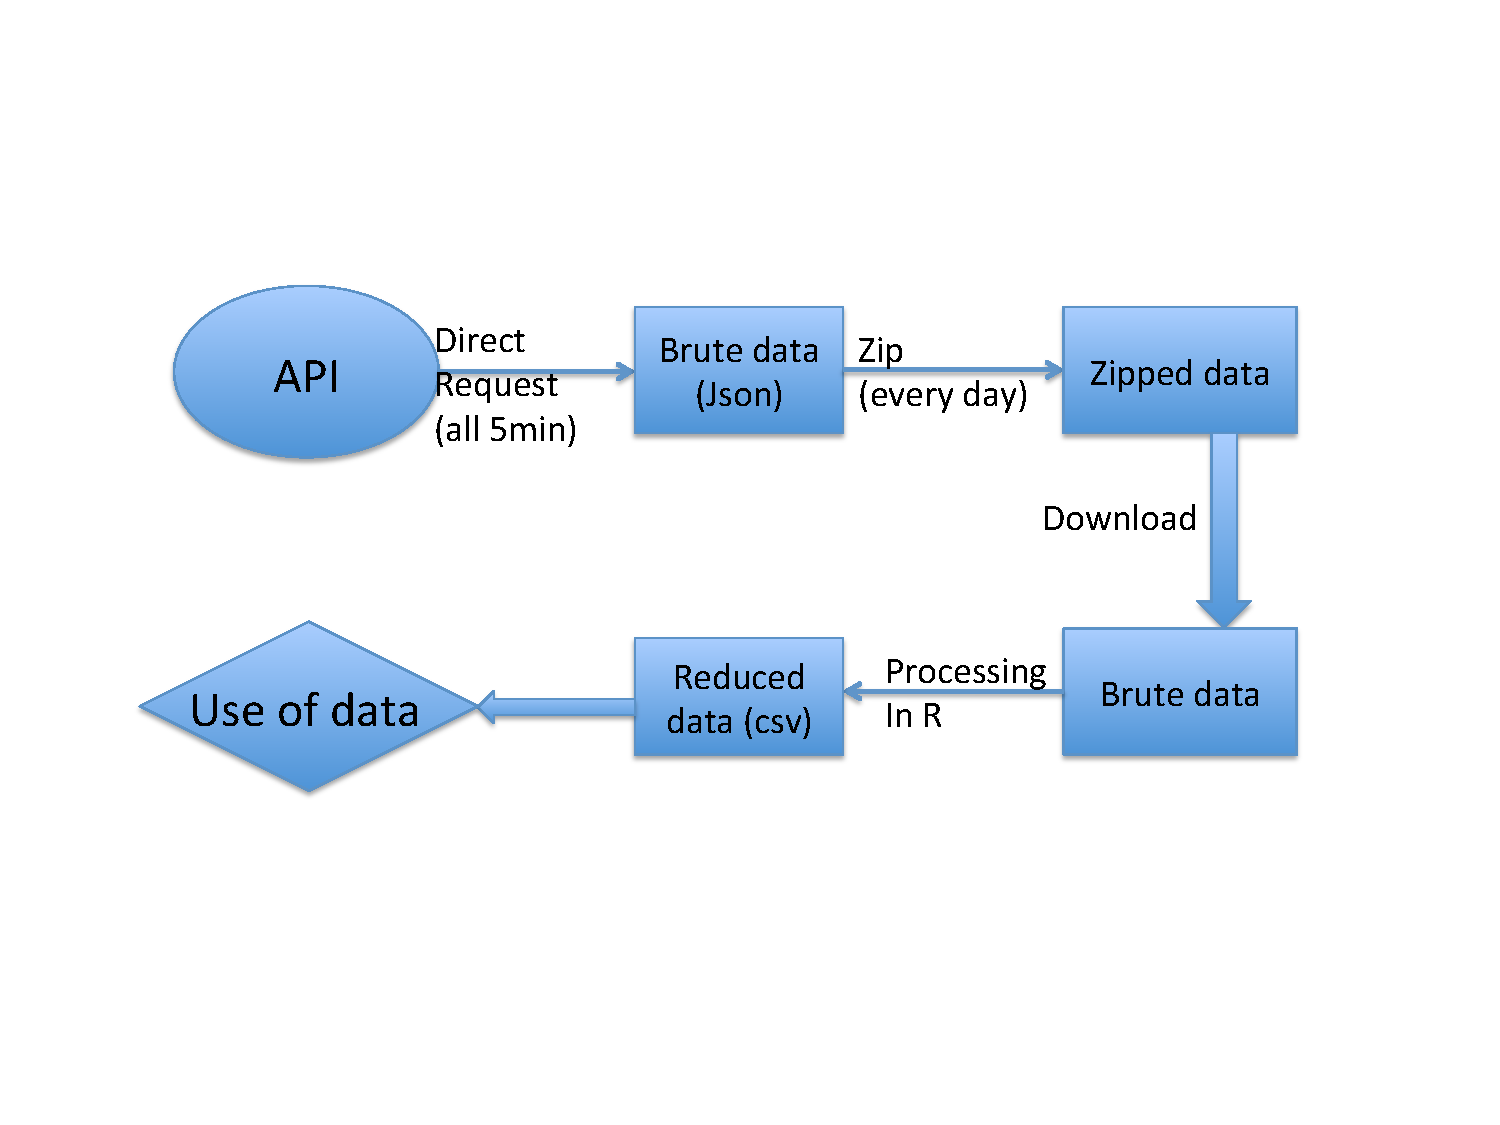
\includegraphics[bb=0bp 100bp 720bp 540bp,scale=0.45]{data}\hfill{}


\lyxframeend{}\section{Statistical analysis}


\lyxframeend{}\lyxframe{Visualisation: mobility patterns}

\hfill{}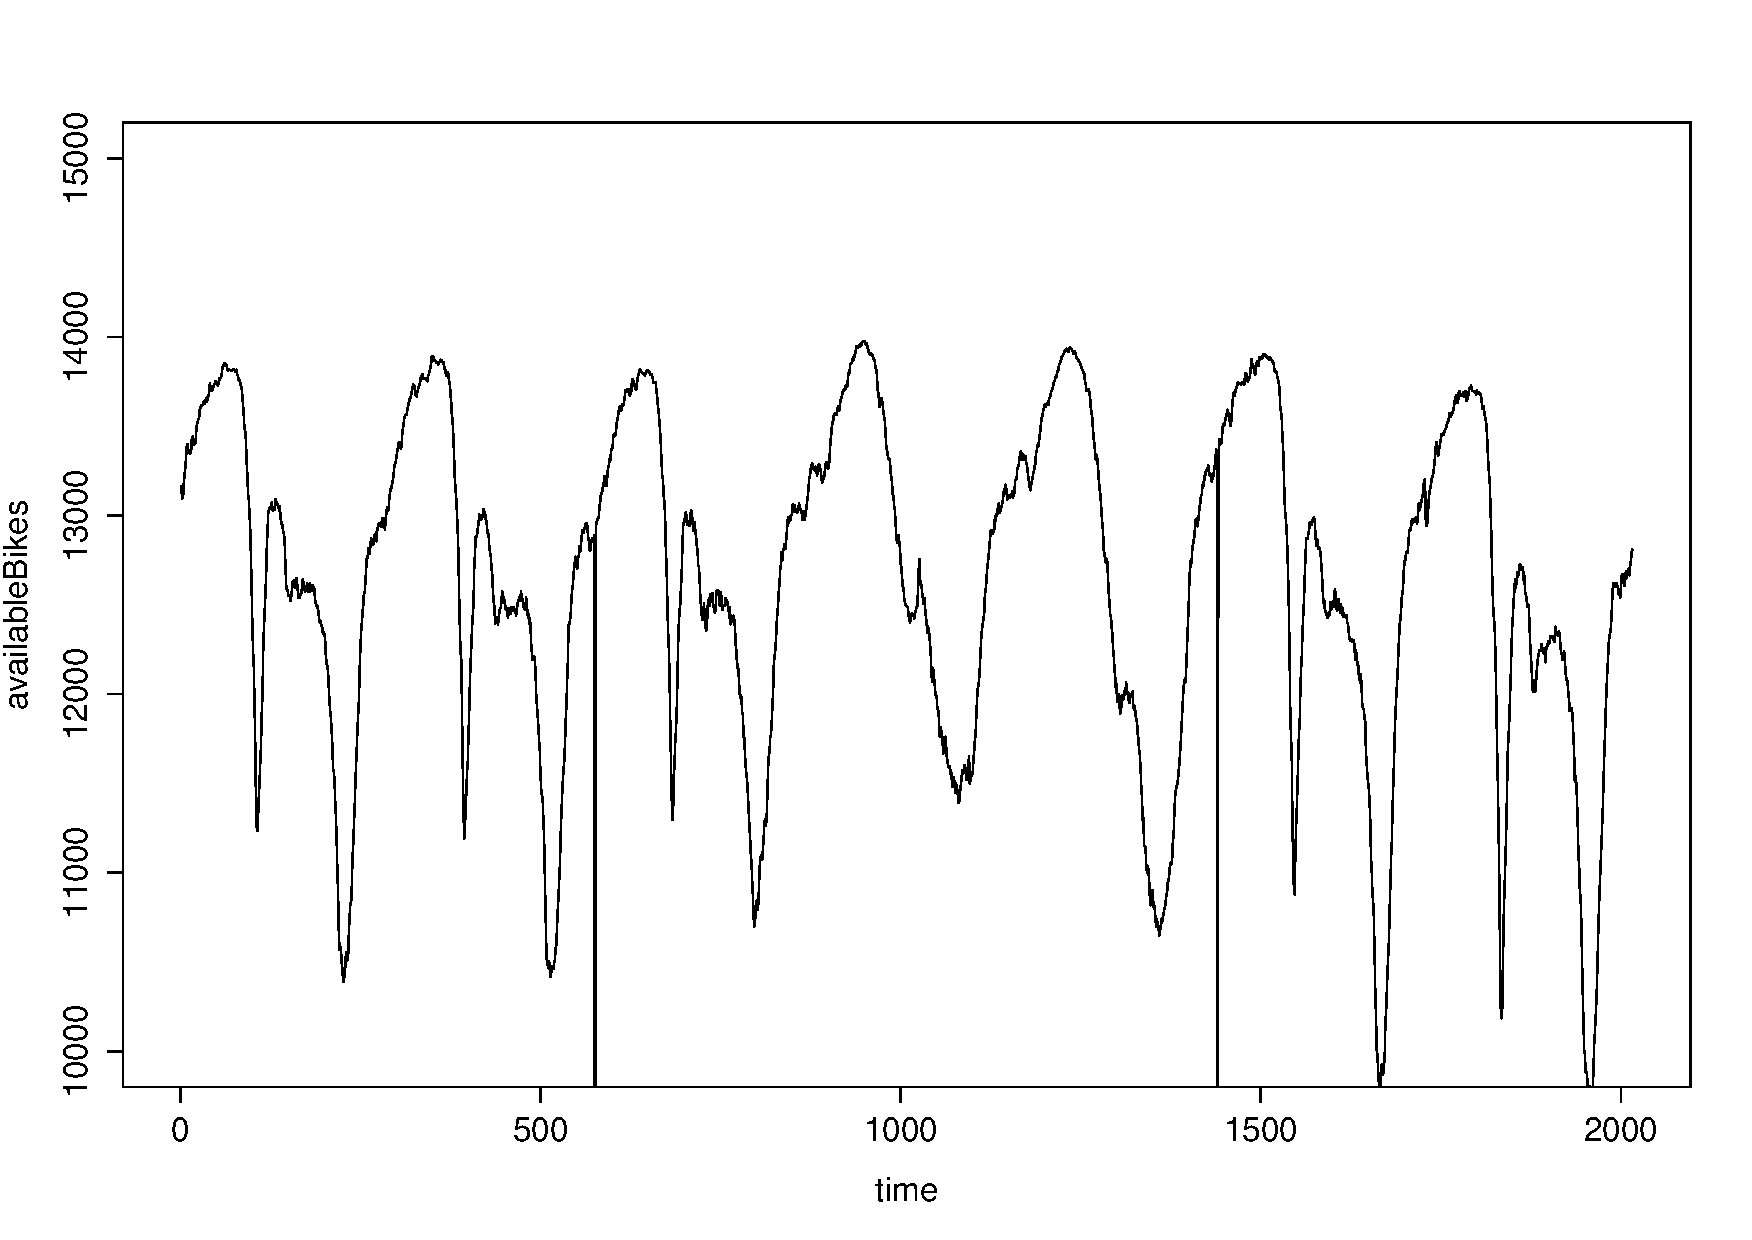
\includegraphics[scale=0.3]{/Users/Juste/Documents/ComplexSystems/CityBikes/Results/Visu/availableBikes}\hfill{}


\lyxframeend{}\lyxframe{Visualisation: heatmaps}

\hfill{}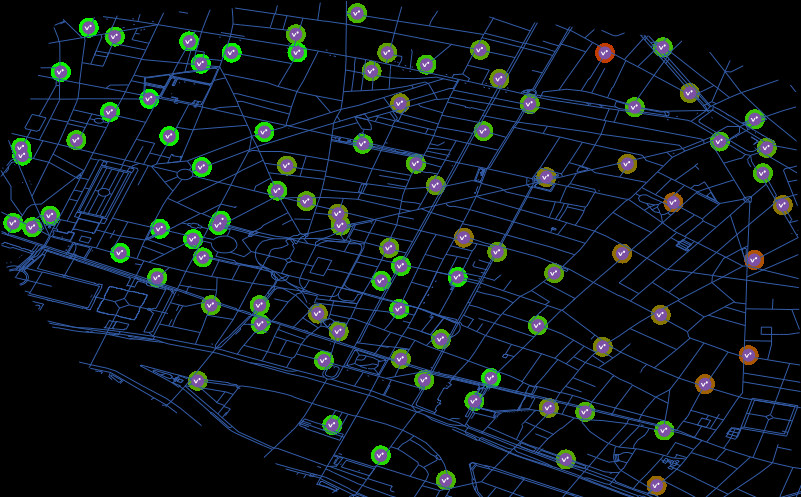
\includegraphics[scale=0.18]{/Users/Juste/Documents/ComplexSystems/CityBikes/Results/Views/lfmidnight}\hfill{}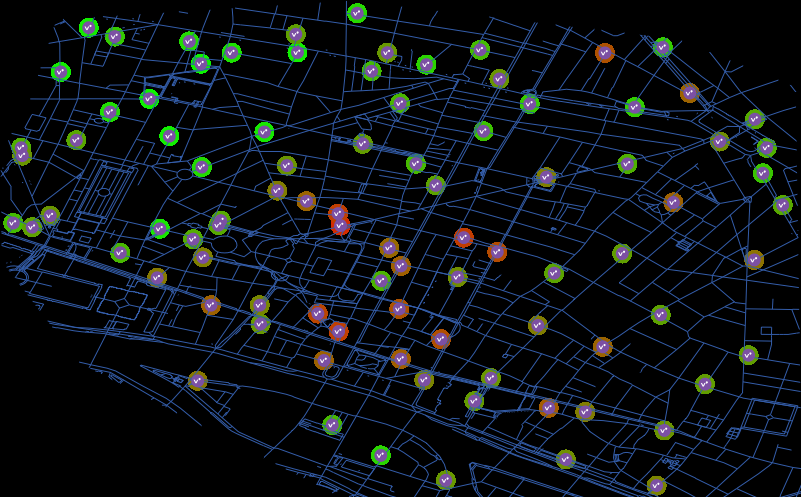
\includegraphics[scale=0.18]{/Users/Juste/Documents/ComplexSystems/CityBikes/Results/Views/lfMidday}\hfill{}


\lyxframeend{}\lyxframe{Extraction of patterns: clustering time-series}

\vfill{}

\begin{itemize}
\item Aim: extract typical use patterns (more characteristic: difference
week/weekends)
\end{itemize}
\vfill{}

\begin{itemize}
\item First sampling of time series, then kmeans (\cite{warren2005clustering})
on sampled series of all stations for a day: gives a reduced representation
of each day
\end{itemize}
\vfill{}

\begin{itemize}
\item Clustering on days to isolate patterns
\end{itemize}
\vfill{}



\lyxframeend{}\lyxframe{Clustering process: role of sampling}

\hfill{}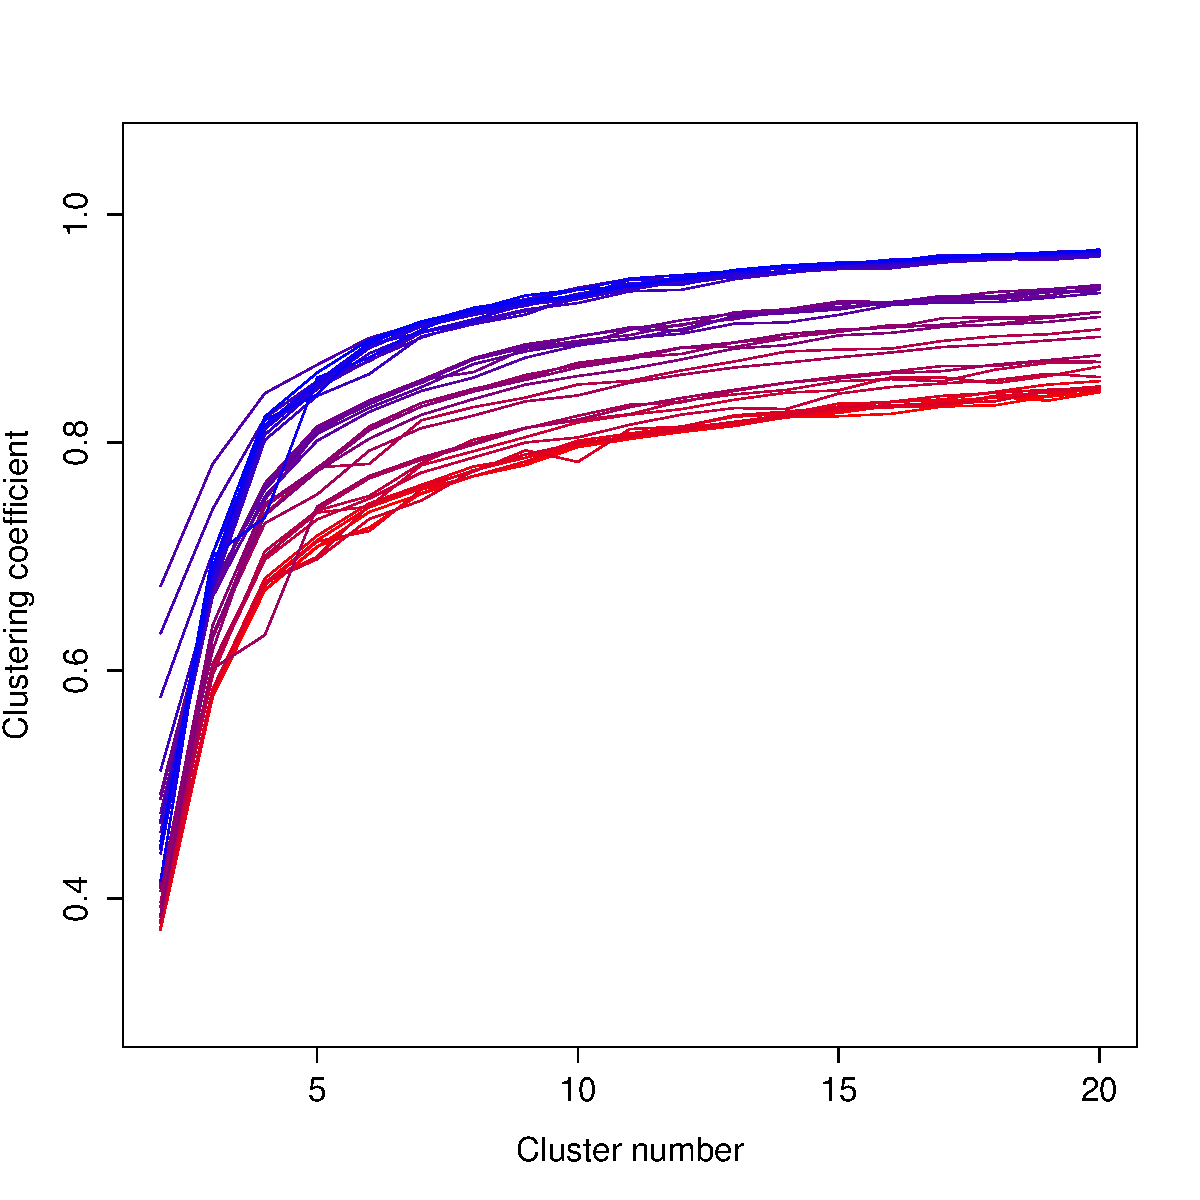
\includegraphics[scale=0.22]{/Users/Juste/Documents/ComplexSystems/CityBikes/Results/Clustering/clusterNumber}\hfill{}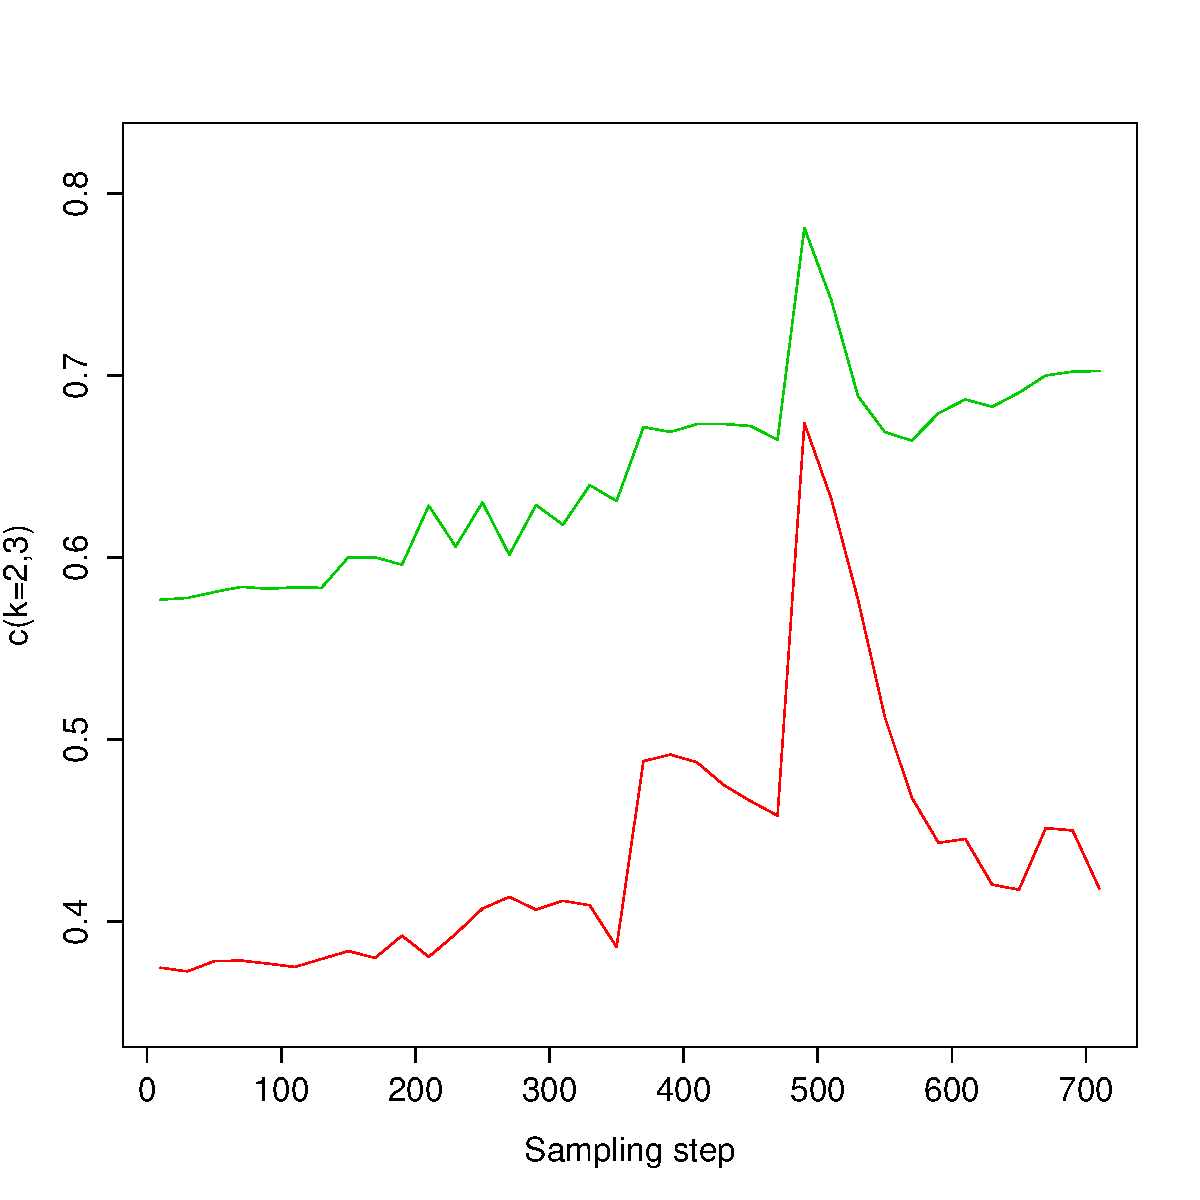
\includegraphics[scale=0.26]{/Users/Juste/Documents/ComplexSystems/CityBikes/Results/Clustering/infoLoss}\hfill{}


\lyxframeend{}\lyxframe{Clustering: results}

\hfill{}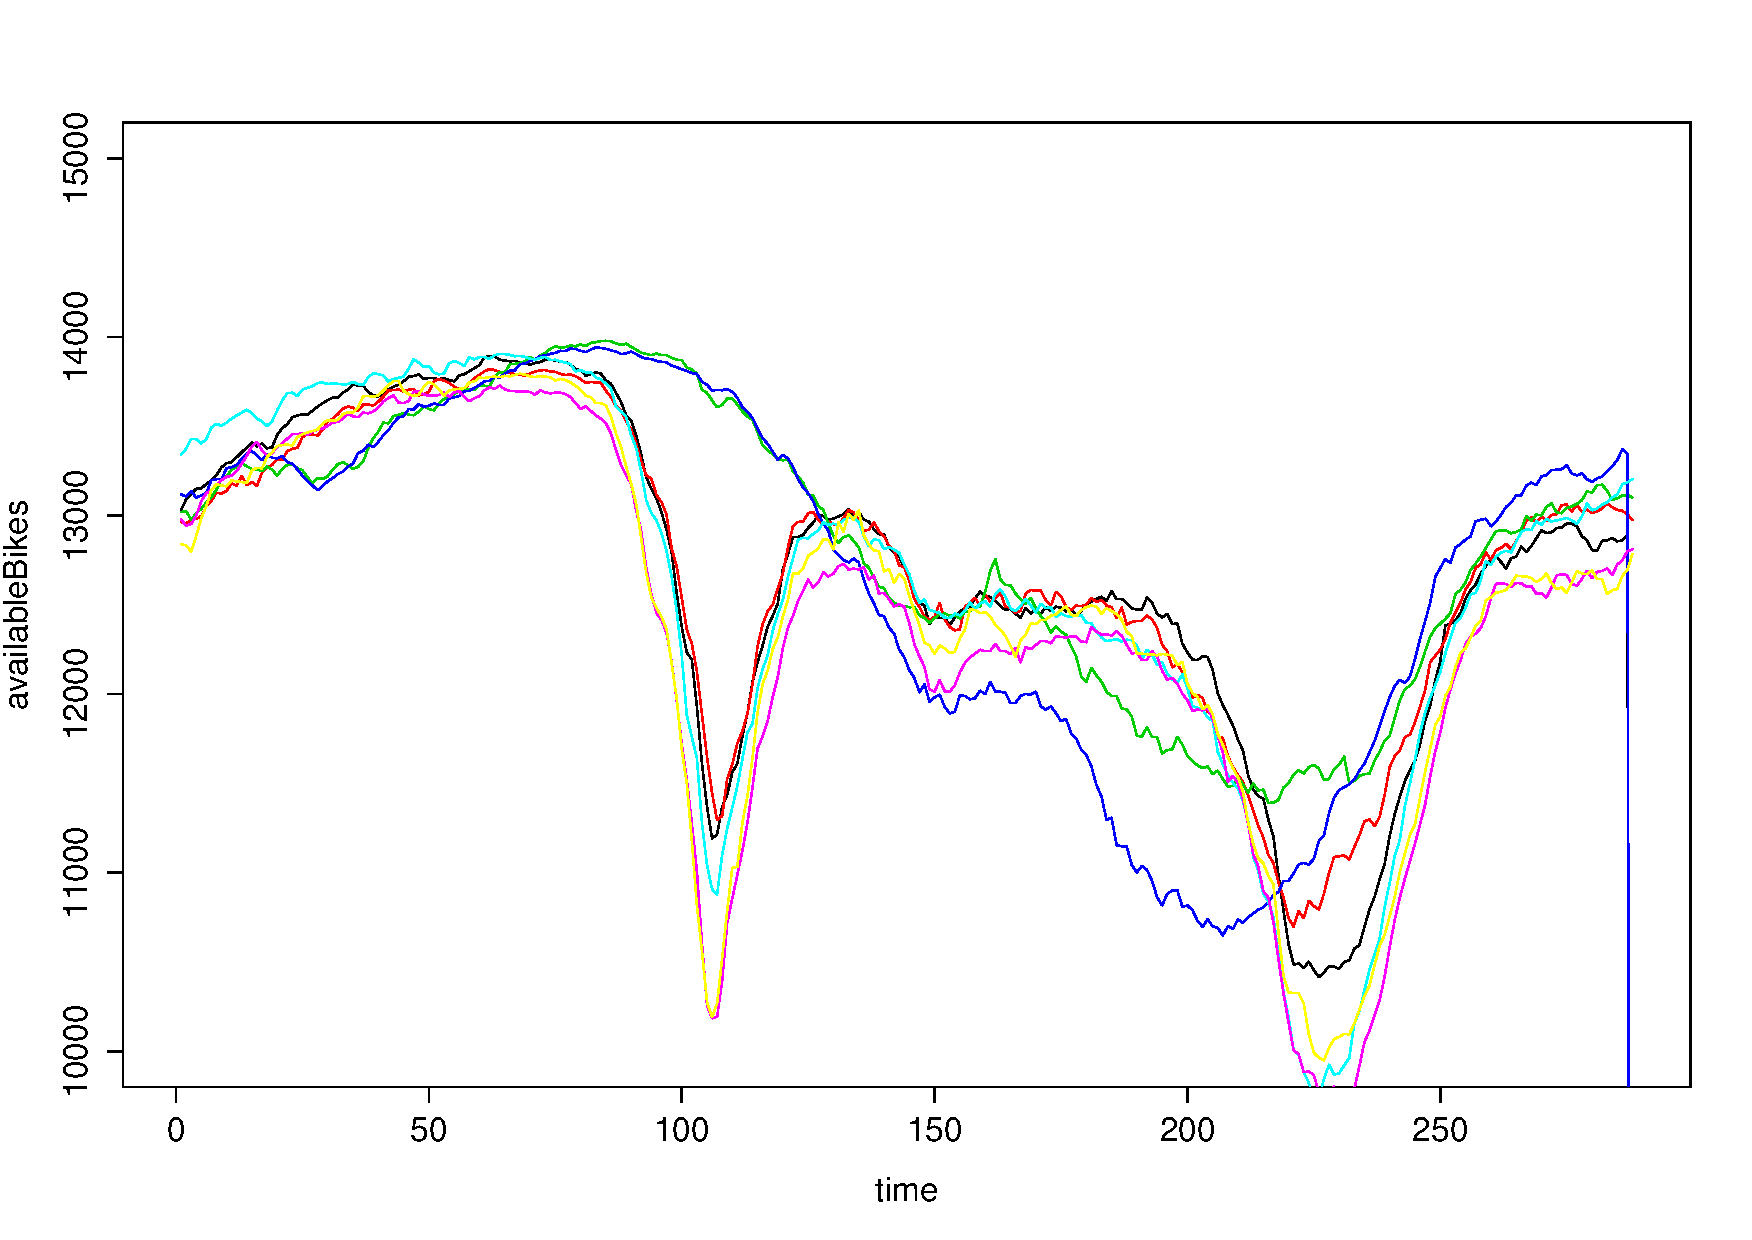
\includegraphics[scale=0.18]{/Users/Juste/Documents/ComplexSystems/CityBikes/Results/Clustering/week}\hfill{}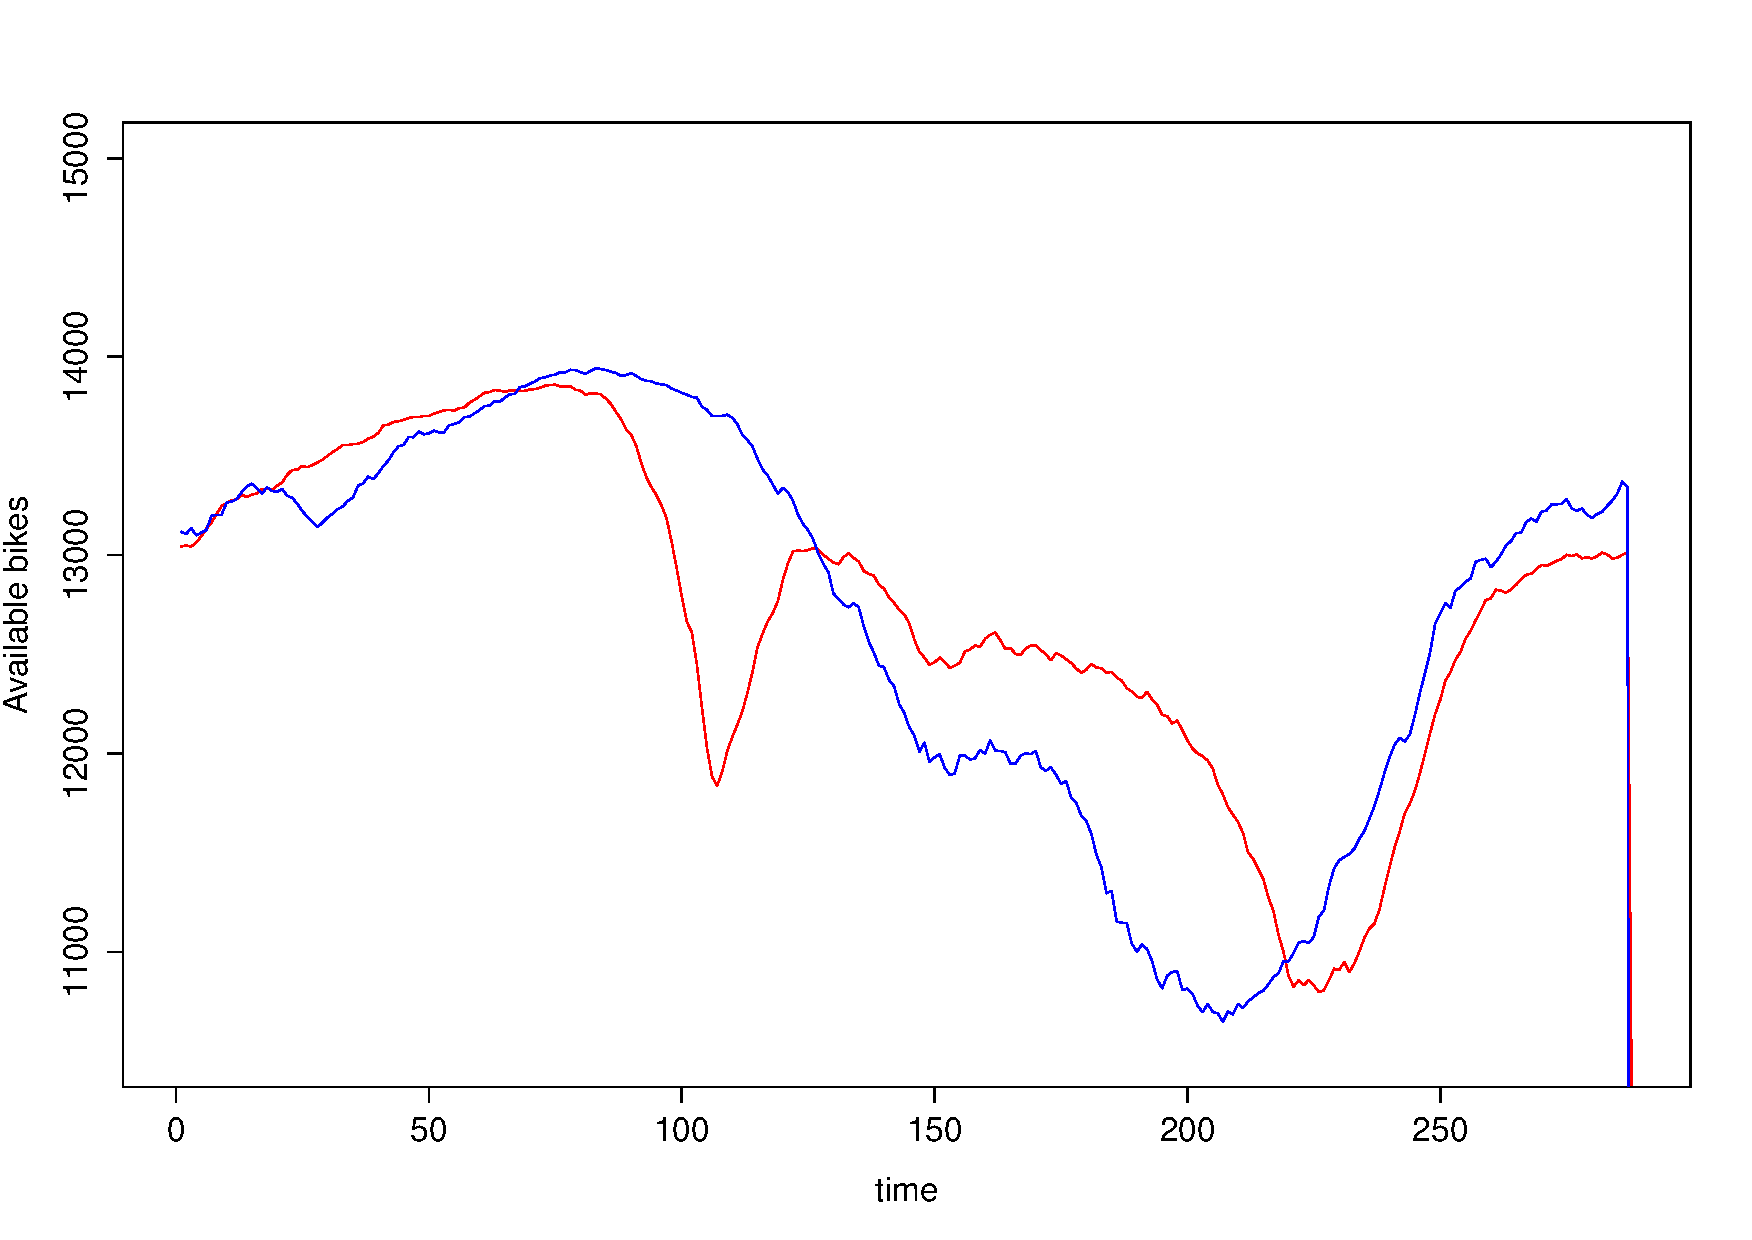
\includegraphics[scale=0.18]{/Users/Juste/Documents/ComplexSystems/CityBikes/Results/Clustering/curves}\hfill{}


\lyxframeend{}\lyxframe{Inference of Origin/destinations in urban mobility}

\vfill{}

\begin{itemize}
\item Core of the parametrisation of the ABM, but also problem with its
intrinsic value (\cite{leurent2006modelisation} )
\end{itemize}
\vfill{}

\begin{itemize}
\item Gaussian kernels non-parametric estimation (\cite{tsybakov2004introduction})
with package kernlab (\cite{karatzoglou2004kernlab}). With $(d_{i}(t))$
real arrivals at $(\vec{x}_{i}(t))$, $D(t)$ spatial field is given
by
\end{itemize}
\[
[D(t)](\vec{x})=\frac{1}{K}\sum_{i}d_{i}(t)\cdot exp(\frac{\left\Vert \vec{x}-\vec{x}_{i}\right\Vert }{2\sigma^{2}})
\]


\vfill{}



\lyxframeend{}\lyxframe{Example}

\hfill{}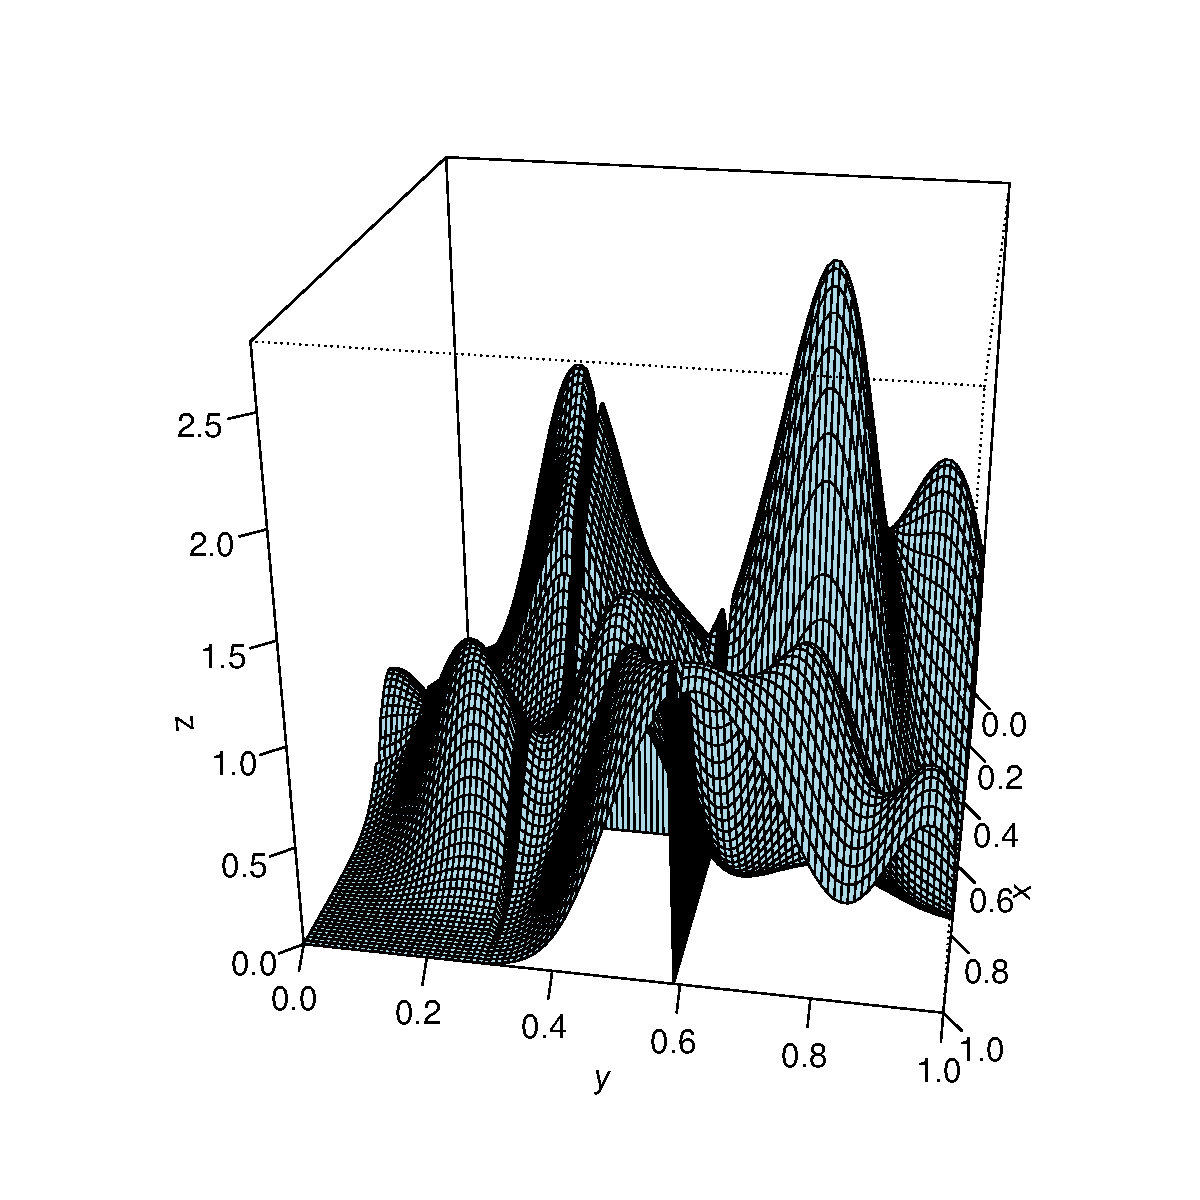
\includegraphics[scale=0.4]{/Users/Juste/Documents/ComplexSystems/CityBikes/Results/Kernel/example}\hfill{}


\lyxframeend{}\lyxframe{Mapping cumulated flows}

\hfill{}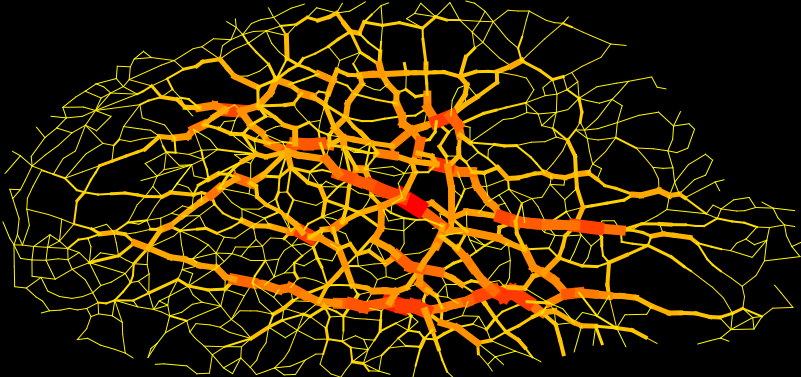
\includegraphics[scale=0.4]{/Users/Juste/Documents/ComplexSystems/CityBikes/Results/Mapping/BikingFlows}\hfill{}


\lyxframeend{}\lyxframe{Use of TE methods ?}

\vfill{}

\begin{itemize}
\item Idea: evaluate effect of redistribution procedure
\end{itemize}
\vfill{}

\begin{itemize}
\item Docking stations are individuals, a treatment is a given area (day
with redistribution gives treated, without redistribution is control
(but for a similar day; use of clustering ?)). Then do a meta-analysis
on all areas.
\end{itemize}
\vfill{}

\begin{itemize}
\item Problem: not even implementable; problem of finding redistributed
area, size of areas, etc
\end{itemize}
\vfill{}



\lyxframeend{}\lyxframe{Conclusion}

\vfill{}

\begin{itemize}
\item Unfortunately did not go so far as expected. However good results
and powerful parametrisation for the ABM
\end{itemize}
\vfill{}

\begin{itemize}
\item We can argue that these data were ``enough'' but still claim for
a broader opening (since yesterday: www.data.gouv.fr ! )
\end{itemize}
\vfill{}



\lyxframeend{}

\begin{frame}[allowframebreaks]
\frametitle{References}

\bibliographystyle{apalike}
\bibliography{/Users/Juste/Documents/Cours/TheoreticalAnalysisComplexSystems/Project/Biblio/biblio,/Users/Juste/Documents/Cours/TheoreticalAnalysisComplexSystems/Project/Biblio/TransportationSystemSafety,/Users/Juste/Documents/ComplexSystems/CityBikes/Biblio/bibtex,/Users/Juste/Documents/ComplexSystems/Biblio/Culture/BibTex/culture,/Users/Juste/Documents/ComplexSystems/Biblio/BibTeX/global}


\end{frame}


\lyxframeend{}\lyxframe{Questions}

{\LARGE \hfill{}}{\Huge ?}{\LARGE \hfill{}\hfill{}}{\LARGE \par}


\lyxframeend{}
\end{document}
